% Ce chapitre repose sur :
%   DOC: s20, s22, s23, s51
%   OBS: REL-IPP.O03, REL-IPP.R12
%   HYP: (aucun)
%   CHI: ablation-comparaisons-variante-a, ablation-ecart-complet, ablation-ecart-variante-a, ablation-ecart-variante-c, ablation-f-variante-a, ablation-f-variante-c
%   CHI: balayage-points, balayage-points-f-parfaite, baseline-f-mesure, blocage-rapport-substitution, collision-adresse-paires, collision-adresse-rappel
%   CHI: collision-adresse-retrouvees, collision-date-naissance-paires, collision-date-naissance-rappel, collision-date-naissance-retrouvees, collision-groupes-nom, collision-groupes-piece
%   CHI: collision-piece-absente-paires, collision-piece-absente-rappel, collision-piece-absente-retrouvees, collision-prenom-compose-paires, collision-prenom-compose-rappel, collision-prenom-compose-retrouvees
%   CHI: collision-telephone-paires, collision-telephone-rappel, collision-telephone-retrouvees, collision-translitteration-paires, collision-translitteration-rappel, collision-translitteration-retrouvees
%   CHI: collision-vides-piece, comparaisons-modele, f-mesure-seuil-retenu, grappes-exactes-global, grappes-exactes-restreint, identifiants-distincts
%   CHI: onglets-recherche, paires-candidates, paires-possibles, precision-seuil-retenu, qualite-colonne-vide, qualite-colonnes
%   CHI: qualite-colonnes-incompletes, rappel-seuil-retenu, regles-blocage, regles-blocage-prevues, regles-blocage-union-reduite, seuil-retenu
%   CHI: sur-fusionnes-global, vt-paires-injectees, vt-paires-presentes
%   SER: (aucune)
%   SECTIONS: 5
\chapter{Qualité des données et rapprochement d'identités}\label{chap:qualite}

Les données de la chaîne portent des défauts injectés, et la question traitée est de savoir ce que
les contrôles en retrouvent. La plupart des défauts se voient sur une ligne seule. Les doublons
d'identité demandent de comparer les fiches deux à deux, ce que fait un rapprochement probabiliste
évalué contre la vérité terrain du générateur.

\section{Les contrôles de qualité de la chaîne}

Deux contrôles de qualité s'ajoutent à la quarantaine (section~\ref{sec:quarantaine}), et chacun a
attrapé des défauts précis. Le premier suit la complétude colonne par colonne. Un agrégat calcule
le taux de renseignement de \chiffre{qualite-colonnes} colonnes de la couche intermédiaire.
Parmi elles, \chiffre{qualite-colonnes-incompletes} sont renseignées à moins de cent pour cent, et
\chiffre{qualite-colonne-vide} ne l'est jamais, parce que le service ne la remplit pas. Les colonnes
les moins remplies sont les téléphones supplémentaires et les champs de liste d'attente, ce qui va
avec un usage où le premier numéro suffit.

Le second contrôle est la collision exacte, qui compte les fiches partageant exactement certains
champs. Elle trouve \chiffre{collision-groupes-nom} groupes de fiches qui partagent nom, premier nom
de famille et date de naissance, et \chiffre{collision-groupes-piece} groupes qui partagent une
pièce d'identité. Le tableau de bord affiche ces décomptes pour décider d'une campagne de fusion
d'identités et du critère à traiter d'abord.

Le second critère ne voit pas les
\chiffre{collision-vides-piece} fiches sans pièce d'identité, et il ne peut pas se prononcer sur
elles. L'agrégat porte donc, pour chaque critère, le nombre de fiches examinées et le nombre de
fiches à valeur vide. Aucun de ces contrôles ne corrige les données : la complétude mesure, la quarantaine met de côté et
la collision compte. Une correction automatique effacerait la trace du défaut, qui est ici l'objet
du travail.

\section{Le problème des doublons dans un fichier patient}

Une même personne qui porte deux identifiants patient est un défaut ordinaire des fichiers
hospitaliers, et il coûte des deux côtés. Un antécédent saisi sous le premier identifiant reste
invisible au praticien qui ouvre le second. Deux dossiers se facturent à part, deux créances
naissent, et le recouvrement se dégrade sans qu'aucune ligne soit fausse.

Le logiciel du service reconnaît lui-même le problème. Son écran de recherche d'identifiant porte \chiffre{onglets-recherche} onglets, dont deux interrogent un index maître des patients, et l'un d'eux propose une
recherche pondérée\releve{REL-IPP.O03}. Les résultats portent en dernière colonne une
probabilité\releve{REL-IPP.R12}. Le produit admet ainsi qu'une même personne peut y figurer
plusieurs fois, et que l'égalité exacte des champs ne suffit pas à la retrouver. La Cour des
comptes relève elle aussi l'attribution de plusieurs identifiants au même patient, et recommande
d'enregistrer la pièce d'identité \cite{s20}.

Les deux erreurs possibles n'ont pas le même coût. Réunir à tort deux personnes mêle leurs dossiers
médicaux, et l'erreur est difficile à défaire une fois les épisodes rattachés. Manquer un doublon
laisse le fichier dans l'état où il était déjà. Les choix de seuil qui suivent découlent de cet
écart.

Un doublon n'est pas une ligne fausse. Les deux fiches sont valides prises séparément, et aucun
contrôle d'entrée ne peut les rejeter. Le défaut n'existe qu'entre elles, et le trouver demande de
comparer les fiches deux à deux.

\section{Le modèle de rapprochement et sa mise en œuvre}

Le rapprochement compare deux fiches champ par champ, donne à chaque accord ou désaccord un poids
appris sur les données, et additionne ces poids. Il suit le modèle de Fellegi-Sunter, que la
bibliothèque employée implémente \cite{s22} et dont la documentation du projet désigne l'exposé de
référence \cite{s23}. Les poids s'estiment sans aucun couple étiqueté, ce qui permet d'utiliser la
méthode sur un fichier réel, où la vérité n'est pas connue.

Un accord sur un champ rare, comme le numéro de pièce d'identité, pèse ainsi bien plus qu'un accord
sur la ville. Le téléphone, parfois rempli d'un numéro inventé (chapitre~\ref{chap:jeu-de-donnees}),
reçoit un poids faible. Le poids total d'une paire se convertit en probabilité, comme la colonne du
même nom à l'écran de recherche du logiciel. Le calcul des poids et l'hypothèse qu'il suppose sont
détaillés en section~\ref{sec:complements-modele}.

Les valeurs sont normalisées avant toute comparaison : passage en minuscules, retrait des accents
et de la ponctuation. Une seconde variante trie aussi les mots d'un champ, ce qui absorbe
l'inversion d'un prénom composé. Une valeur vide reste vide.

Comparer toutes les paires est impossible, car les \chiffre{identifiants-distincts} fiches de version
courante en forment \chiffre{paires-possibles}. Le blocage ne compare donc que les paires qui
s'accordent déjà sur un critère simple, par exemple le même nom de famille et le même téléphone.
Les \chiffre{regles-blocage} règles de blocage retiennent ainsi \chiffre{paires-candidates} paires candidates, et leur
détail est donné en section~\ref{sec:complements-modele}.

Le rappel est la part des doublons de la vérité terrain qu'une étape retrouve \cite{s51}. Une
quatrième règle a été ajoutée aux \chiffre{regles-blocage-prevues} prévues, parce que l'union des \chiffre{regles-blocage} donne au blocage son
rappel maximal pour \chiffre{paires-candidates} paires. La meilleure union de \chiffre{regles-blocage-union-reduite} règles qui
atteignait ce rappel produisait \chiffre{blocage-rapport-substitution} fois plus de paires. Le modèle estimé porte
\chiffre{comparaisons-modele} comparaisons de champs, chacune en niveaux du plus strict au plus
permissif.

Les champs d'identité du jeu ne peuvent pas désigner une personne réelle, parce que le jeu de
données est publié. Aucun champ synthétique ne prend une valeur possible dans son espace réel : un
numéro de téléphone tiré sur un préfixe attribué serait le numéro de quelqu'un. L'impossibilité
tient à la structure, comme une longueur qu'aucun plan de numérotation n'admet, et non à une plage
aujourd'hui libre. Un contrôle bloquant le vérifie champ par champ. Il porte sur les identifiants,
qui désignent une personne ou un compte, et non sur les noms, les voies ou les villes, qui la
décrivent.

\section{Évaluation contre la vérité terrain}

Contre la vérité terrain, le modèle retrouve tous les doublons sans fusion à tort, et ce score
parfait dit surtout que le jeu sépare très bien les deux populations. Le générateur enregistre les
\chiffre{vt-paires-injectees} paires de doublons qu'il injecte. Une paire dont une fiche est partie
en quarantaine ne peut pas être retrouvée, et l'évaluation porte donc sur les
\chiffre{vt-paires-presentes} paires dont les deux fiches sont présentes.

Au seuil retenu de \chiffre{seuil-retenu}, la précision du modèle vaut
\chiffre{precision-seuil-retenu} : c'est la part des paires déclarées doublons qui le sont dans la
vérité terrain \cite{s51}. Le rappel du modèle vaut \chiffre{rappel-seuil-retenu}. La F-mesure,
moyenne harmonique des deux, vaut \chiffre{f-mesure-seuil-retenu} \cite{s51}. Les trois sont
mesurées au niveau de la paire.

Le balayage compte \chiffre{balayage-points} seuils, et \chiffre{balayage-points-f-parfaite} d'entre
eux donnent la même F-mesure de \chiffre{f-mesure-seuil-retenu} (voir
figure~\ref{fig:precision-rappel}). Le seuil ne fait donc presque rien, parce que les paires vraies
et les paires fausses sont très séparées. La section~\ref{sec:limites-rapprochement} montre ce qui
arrive quand cette séparation disparaît. Chaque point de la figure est un seuil du balayage, et le
point carré est la référence par collision exacte, qui ne dépend d'aucun seuil.

\begin{figure}[htbp]
\centering
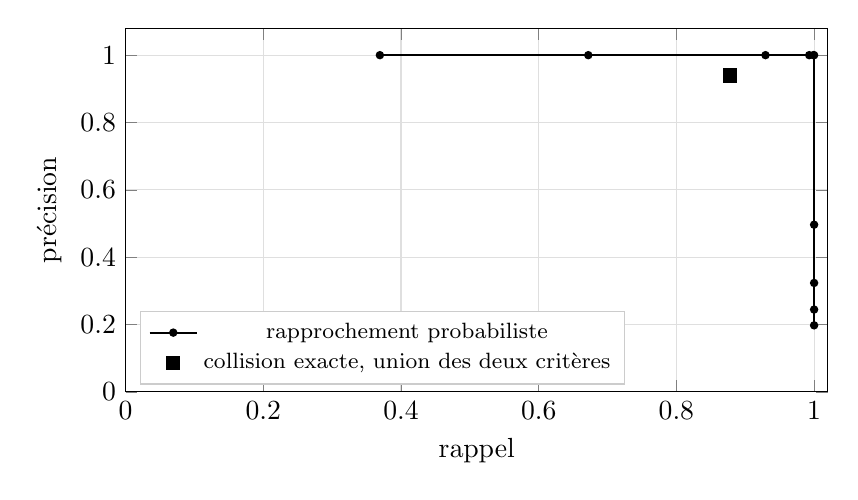
\begin{tikzpicture}
\begin{axis}[
  width=10.5cm, height=6.2cm,
  xlabel={rappel}, ylabel={précision},
  xmin=0, xmax=1.02, ymin=0, ymax=1.08,
  xtick={0,0.2,0.4,0.6,0.8,1.0}, ytick={0,0.2,0.4,0.6,0.8,1.0},
  grid=major, grid style={gray!25},
  every axis plot/.append style={thick},
  legend style={at={(0.02,0.02)}, anchor=south west, font=\footnotesize, draw=gray!40},
]
\addplot[mark=*, mark size=1.1pt, color=black] coordinates {
 (1.0,0.1976) (1.0,0.2445) (1.0,0.3235) (1.0,0.4965) (1.0,1.0)
 (0.9990,1.0) (0.9929,1.0) (0.9294,1.0) (0.6720,1.0) (0.3693,1.0)
};
\addlegendentry{rapprochement probabiliste}
\addplot[only marks, mark=square*, mark size=2.2pt, color=black] coordinates {(0.8779,0.9395)};
\addlegendentry{collision exacte, union des deux critères}
\end{axis}
\end{tikzpicture}
\caption{Précision en fonction du rappel, sur le balayage de seuils}\label{fig:precision-rappel}
\end{figure}

Une métrique de grappe accompagne la métrique de paire, parce qu'une paire manquée casse toute sa
grappe. Sur les identifiants qui ont au moins une paire dans la vérité terrain,
\chiffre{grappes-exactes-restreint} grappes sont retrouvées exactement. Sur toute la population,
singletons compris, \chiffre{grappes-exactes-global} le sont, soit toutes, et
\chiffre{sur-fusionnes-global} fiches sont réunies à tort. Le seuil retenu ne se choisit pas sur la
F-mesure, qui exigerait des étiquettes qu'un service réel n'a pas. Il est placé du côté prudent du
plateau, parce qu'une fusion à tort coûte plus qu'un doublon manqué.

La référence est la collision exacte, qu'un service peut écrire en une requête. Deux fiches y sont
un doublon si elles partagent exactement nom, premier nom de famille et date de naissance, ou
exactement type et numéro de pièce d'identité. Sa F-mesure vaut \chiffre{baseline-f-mesure}, et sa
défaillance se lit variation par variation (voir tableau~\ref{tab:rappel-collision}).

\begin{table}[htbp]
\centering
\caption{Rappel de la collision exacte, par variation injectée}\label{tab:rappel-collision}
\begin{tabular}{@{}p{6.2cm}rrr@{}}
\toprule
Variation injectée & Paires & Retrouvées & Rappel \\
\midrule
téléphone différent & \chiffre{collision-telephone-paires} & \chiffre{collision-telephone-retrouvees} & \chiffre{collision-telephone-rappel} \\
adresse mise à jour & \chiffre{collision-adresse-paires} & \chiffre{collision-adresse-retrouvees} & \chiffre{collision-adresse-rappel} \\
faute de frappe sur la date de naissance & \chiffre{collision-date-naissance-paires} & \chiffre{collision-date-naissance-retrouvees} & \chiffre{collision-date-naissance-rappel} \\
translittération du prénom & \chiffre{collision-translitteration-paires} & \chiffre{collision-translitteration-retrouvees} & \chiffre{collision-translitteration-rappel} \\
prénom composé inversé & \chiffre{collision-prenom-compose-paires} & \chiffre{collision-prenom-compose-retrouvees} & \chiffre{collision-prenom-compose-rappel} \\
\textbf{pièce d'identité absente} & \textbf{\chiffre{collision-piece-absente-paires}} & \textbf{\chiffre{collision-piece-absente-retrouvees}} & \textbf{\chiffre{collision-piece-absente-rappel}} \\
\bottomrule
\end{tabular}
\end{table}

Le rappel y porte sur les \chiffre{vt-paires-presentes} paires présentes, et une paire qui porte
plusieurs variations compte dans chaque ligne qui la concerne. La collision exacte échoue là où le
champ qu'elle utilise manque ou est déformé. Elle retrouve tous les doublons dont seul le téléphone
diffère, parce que ses deux critères ne lisent pas le téléphone. Elle en manque près de la moitié
quand la pièce d'identité manque, et \chiffre{collision-vides-piece} fiches n'en portent aucune.

Le rapprochement probabiliste retrouve les \chiffre{vt-paires-presentes} paires, parce qu'il
additionne ce que chaque champ apporte sans exiger qu'aucun soit présent ou exact. Son intérêt n'est
donc pas un meilleur score moyen. Il se dégrade peu à peu là où la collision exacte s'effondre, et
un fichier réel a justement cette forme : champs manquants, orthographes concurrentes, dates saisies
de travers.

\section{Les limites de l'évaluation}\label{sec:limites-rapprochement}

La vérité terrain vient du générateur, et c'est la limite qui domine les autres. Les
\chiffre{vt-paires-injectees} paires ont été injectées par le projet, avec des déformations qu'il a
choisies : translittération d'un prénom, inversion d'un prénom composé, faute de frappe sur une
date, changement d'adresse ou de téléphone, absence de pièce d'identité. Sur des données réelles,
les déformations seraient plus variées et plus corrélées, et les taux d'absence varieraient d'un
champ et d'une population à l'autre. La proportion de vrais doublons y serait inconnue, alors
qu'elle est ici fixée par construction.

L'ablation mesure ce que le modèle doit aux champs recopiés par le générateur. Quand il crée un
doublon, le générateur recopie le second nom de famille, les noms des parents, le quartier et la
ville, et le modèle apprend à s'y fier. Le tableau~\ref{tab:ablation} compare le modèle complet à
deux variantes : sans les champs recopiés, puis avec en plus l'absence de pièce d'identité
neutralisée.

\begin{table}[htbp]
\centering
\caption{Ablation des champs recopiés par le générateur}\label{tab:ablation}
\begin{tabular}{@{}p{4.6cm}rrr@{}}
\toprule
Variante & Comparaisons & F-mesure & Marge \\
\midrule
modèle complet & \chiffre{comparaisons-modele} & \chiffre{f-mesure-seuil-retenu} & \chiffre{ablation-ecart-complet} \\
sans les champs recopiés & \chiffre{ablation-comparaisons-variante-a} & \chiffre{ablation-f-variante-a} & \chiffre{ablation-ecart-variante-a} \\
les deux retraits cumulés & \chiffre{ablation-comparaisons-variante-a} & \chiffre{ablation-f-variante-c} & \chiffre{ablation-ecart-variante-c} \\
\bottomrule
\end{tabular}
\end{table}

La marge y est l'écart entre le poids le plus faible d'une paire vraie et le poids le plus fort
d'une paire fausse. Positive, elle laisse un seuil séparer les deux populations, et négative, elle
n'en laisse aucun. La F-mesure bouge à peine : elle passe de \chiffre{f-mesure-seuil-retenu} à
\chiffre{ablation-f-variante-c}. La marge passe de \chiffre{ablation-ecart-complet} à
\chiffre{ablation-ecart-variante-a} sans les champs recopiés, puis à
\chiffre{ablation-ecart-variante-c} avec les deux retraits. Une marge négative signifie qu'une paire
fausse est mieux notée qu'une paire vraie, même si le nombre d'erreurs reste faible.

La perfection apparente du rapprochement tient donc en partie à des champs que le générateur a
recopiés. Sur un fichier réel, ces champs ne seraient pas identiques par construction, et la marge
ressemblerait davantage à celle des variantes. La chaîne montre qu'elle sait estimer un modèle sans
étiquettes, bloquer efficacement, évaluer ses résultats et mesurer sa propre fragilité. Elle ne
montre pas qu'un rappel parfait est atteignable sur des données qu'elle n'a pas produites.

\section*{Synthèse}

Les contrôles de qualité ont attrapé les défauts qu'une ligne trahit seule, sans rien corriger. Les
doublons d'identité demandent un rapprochement, qui retrouve toutes les paires de la vérité terrain
là où la collision exacte en manque. Ce score parfait dépend en partie du jeu lui-même, comme
l'ablation le montre. Le chapitre~\ref{chap:outils} présente les outils qui portent la chaîne.
